\documentclass{article}
\usepackage[utf8]{inputenc}
\usepackage[english]{babel}
\usepackage{amsmath}
\usepackage{amsfonts}
\usepackage{amssymb}
\usepackage{amsthm}
\usepackage[basic]{complexity}
\usepackage{tikz}
\usepackage{hyphenat}
\usepackage{graphicx}
\usepackage{mathpazo}
\usepackage{nicefrac}

\usepackage[authoryear]{natbib}

\usepackage{geometry}
\geometry{vmargin = 3cm, hmargin = 3cm}

\usepackage{array}
\newcolumntype{L}[1]{>{\raggedright\let\newline\\\arraybackslash\hspace{0pt}}m{#1}}
\newcolumntype{C}[1]{>{\centering\let\newline\\\arraybackslash\hspace{0pt}}m{#1}}
\newcolumntype{R}[1]{>{\raggedleft\let\newline\\\arraybackslash\hspace{0pt}}m{#1}}

\renewcommand{\arraystretch}{1.15}

\usepackage{tikz}
\usetikzlibrary{automata, positioning, calc, shapes, arrows, fit}
\newcommand{\circled}[1]{\tikz[baseline=(char.base)]{
		\node[shape=circle, draw, inner sep=0.5pt] (char) {#1};}}

\usepackage[unicode=true, bookmarks=false, breaklinks=true, pdfborder={0 0 1},colorlinks=true]{hyperref}
\hypersetup{linkcolor=blue,citecolor=blue,filecolor=blue,urlcolor=blue}


\begin{document}
	\title{Preflib 2.0}
	\author{Simon Rey, Nick Mattei}
	\maketitle
	
	\tableofcontents
	
	\section{Folder Structure}
	
	The folder structure of the project follows that of a typical Django project with one application. In the following we will go through the important files.
	
	\begin{itemize}
		\item preflib
		\begin{itemize}
			\item settings.py: all the inner settings of the project, only change things there if you know what you're doing.
			\item urls.py: general patterns for URL, since there only is one application the file is quite basic. Handlers for errors (500, 404, ...) also are defined there.
			\item wsgi.py: used to link django to the http server, do not modify.
		\end{itemize}
		\item preflibApp
		\begin{itemize}
			\item management/commands
			\begin{itemize}
				\item adddataset.py: management command used to add a dataset to the database.
				\item createmetadata.py: command to generate all the metadata for the datafile in the database.
				\item generatezip.py: generates all the zip files.
				\item initializedb.py: command to be run when setting up the website.
				\item updatepapers.py: update the list of the papers using Preflib according the a bib file.
			\end{itemize}
			\item migrations: inner Django stuff, do not modify.
			\item preflibtools: nothing to do with Django, all the tools used to deal with the data.
			\item static: all the static files that are served by the website.
			\item templates: a template is an html file which can incorporate some Django code to perform some computations in it. This folder contains the general html structure of the website, i.e., all its templates.
			\item templatetags: custom tags that can be used in the templates.
			\item admin.py: define which tables can be accessed on the Django admin page of the website.
			\item apps.py: inner Django stuff, do not modify.
			\item choices.py: several fields in the database have to be selected among a specific list. All the lists that are not worth putting in the database (because they never change for instance) are defined here.
			\item forms.py: the Django representation of the html forms that are used in the website. It is for instance, the login form, some administrative forms...
			\item models.py: all Danjgo objects representing the tables in the database. This is an important file that describes the entire database structure.
			\item scripts.py: some useful scripts, mainly used for management purposes.
			\item urls.py: the URL pattern for the pages available through this app.
			\item views.py: the most important file. The views are functions that are called to render the page requested by the user. This is where all the computations that are done at runtime are described.
		\end{itemize}
		\item manage.py: Python file to run local functions
	\end{itemize}
	
	\section{Database Structure}
	
	In the following, we provide more details about the structure of the database behind Preflib.
	
	\medskip
	
	Let us first go through all the tables present in the database.
	
	\paragraph{\textsc{DataFile}} The most fundamental entity for Preflib is the datafile. The \textsc{DataFile} table contains a reference to all the datafiles that are in Preflib. The table does not contain the data in itself---it is stored in a file and not in the database---but all the relevant information about it: some basic details and datapatch in which the file is.
	
	\paragraph{\textsc{DataPatch}} The datapatch is the first level of classification of the datafile. It contains several datafile of different datatype. All the datafiles are based on the same preferences but the representation, the datatype, is different.
	
	\paragraph{\textsc{DataSet}} A dataset is a collection of datapatches. The datapatches will typically represent different years of the same election.
	
	\paragraph{\textsc{DataProperty}} A dataproperty is an additional information about a given datafile. It can have to do about the general properties of the data (number of candidates...) or about some more specific structure of the data (single-peakedness...).
	
	\paragraph{\textsc{Metadata}} The \textsc{Metadata} table stores all the different metadata available in the system. Their values are in the \textsc{DataProperty} table.
	
	\paragraph{\textsc{Paper}} This table stores the information about the papers which are using Preflib.
	
	\paragraph{\textsc{UserProfile}} All the informations about the users that are not in the Django User class are present in this table.
	
	\paragraph{\textsc{Log}} Logs of what is happening in the inside are gathers in this table.
	
	\medskip
	
	The following figure summarizes the links between the different tables and presents all the elements present in the tables.
	
	\begin{center}
		\resizebox{\linewidth}{!}{
		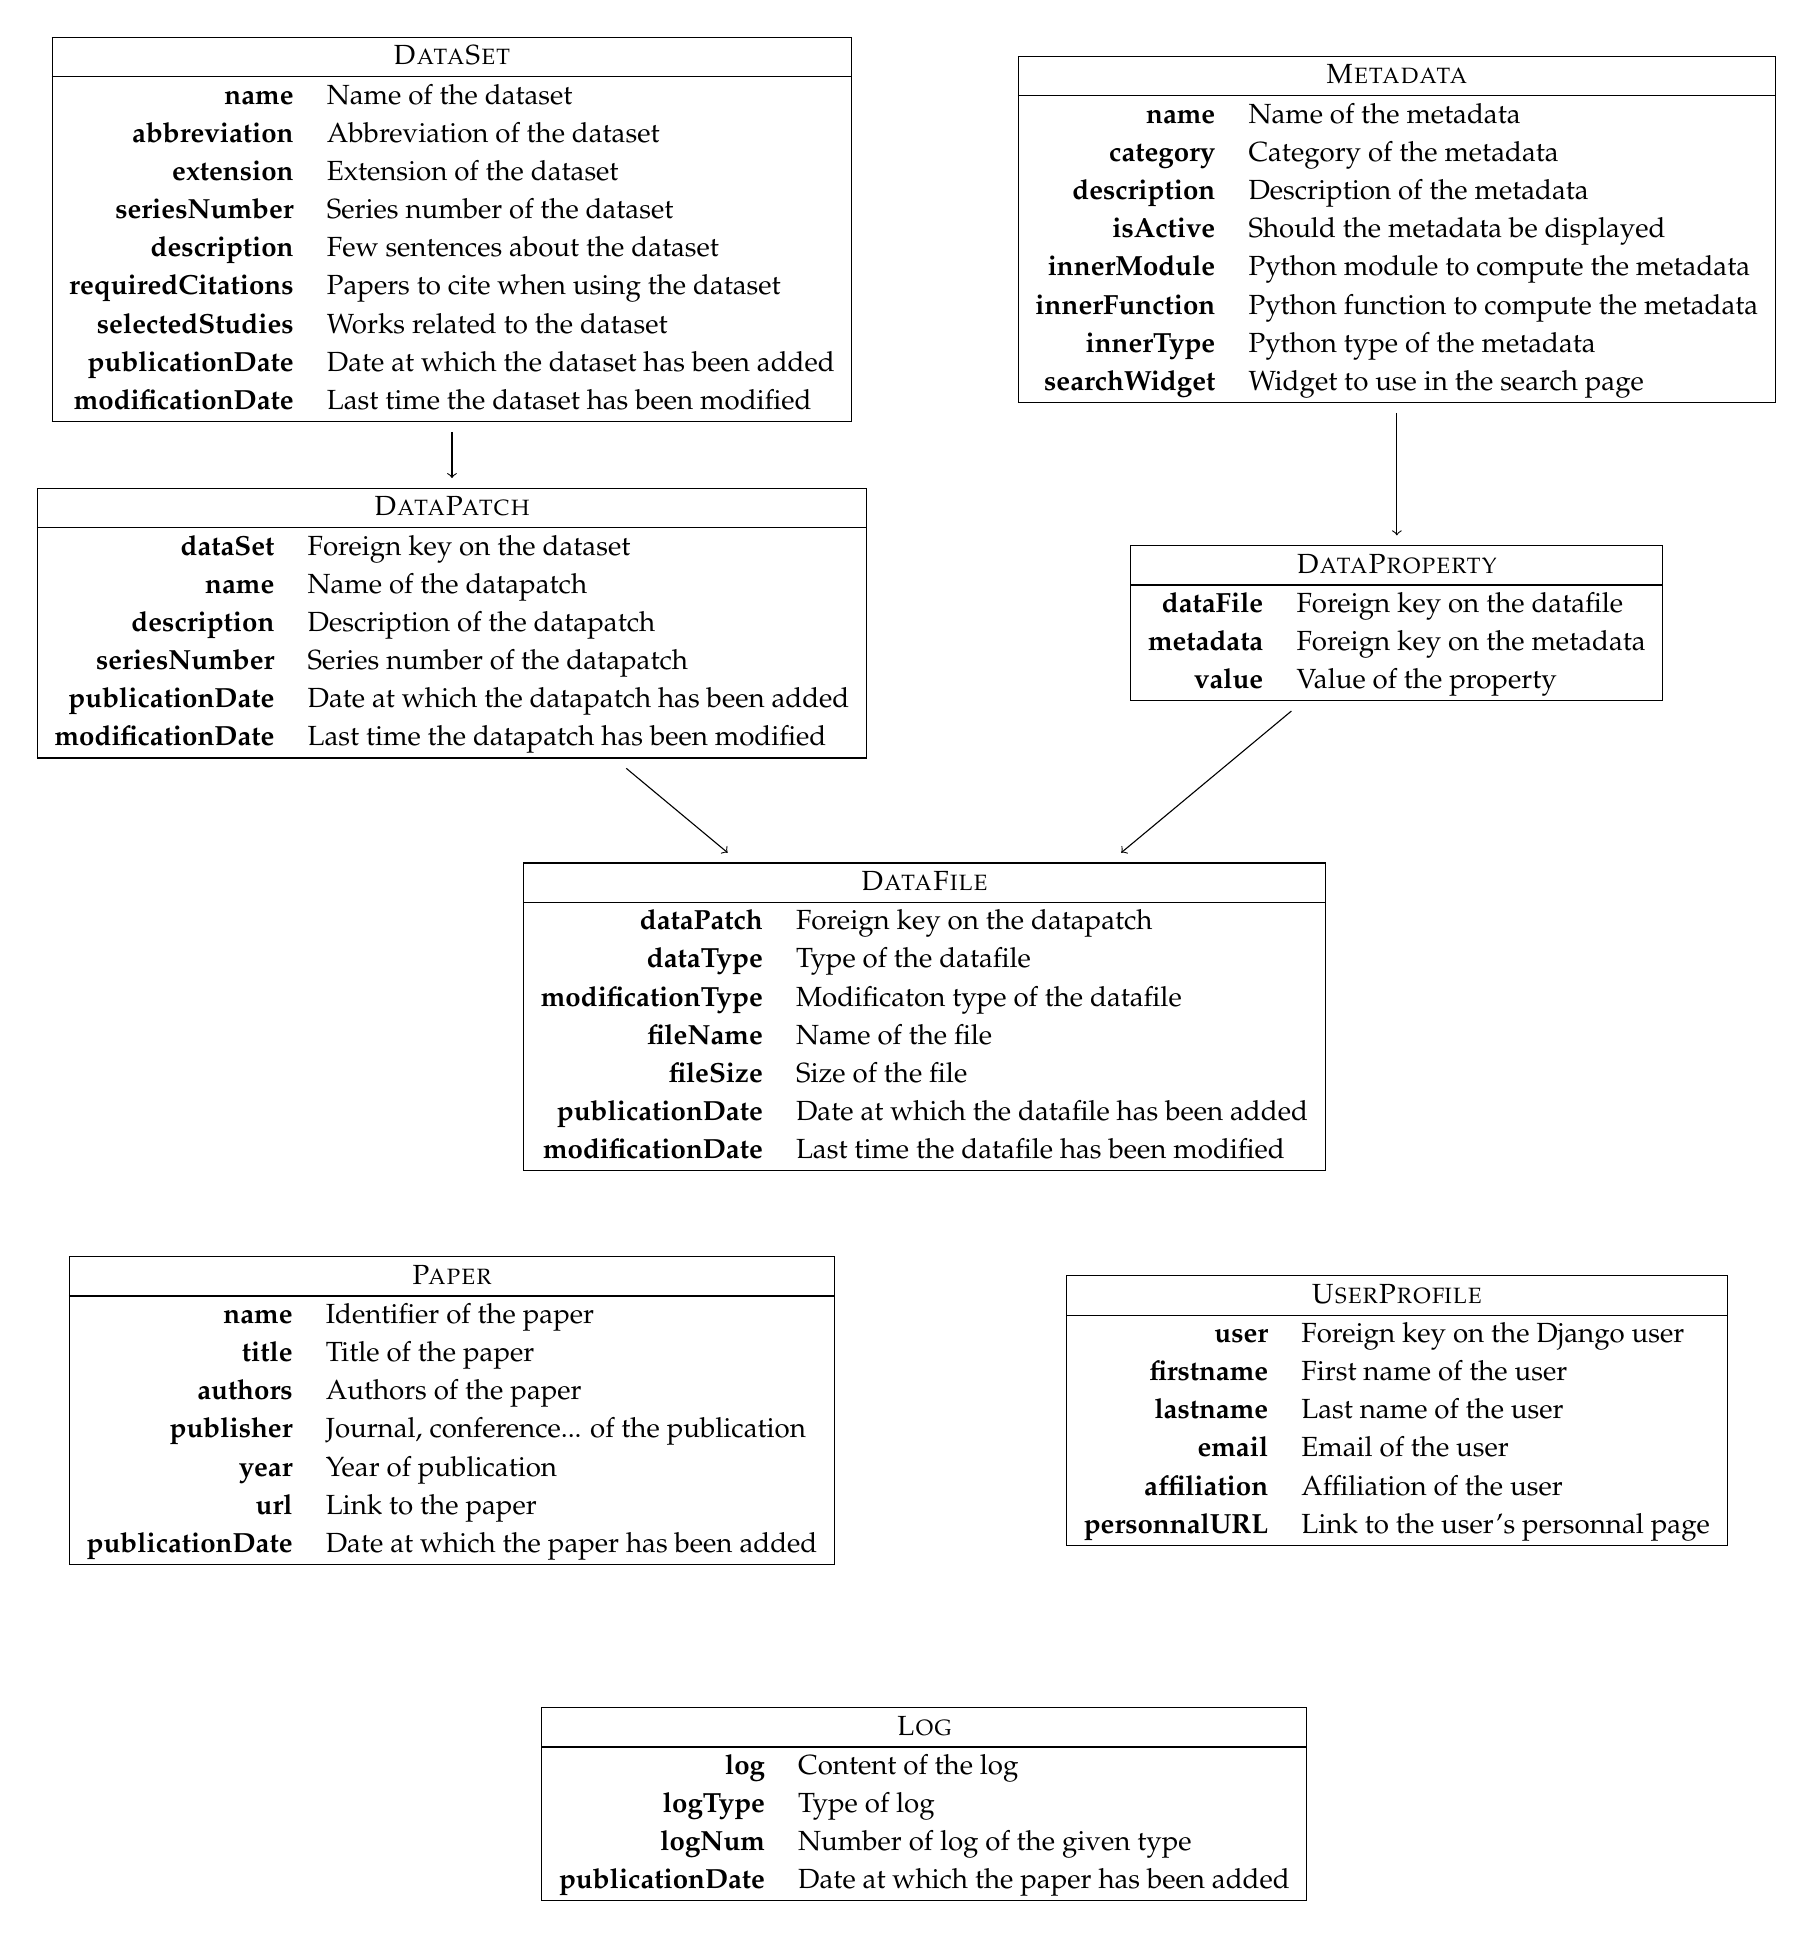
\begin{tikzpicture}
			\node[] (dataset) at (0, 0) {\begin{tabular}{|rl|}
					\hline
					\multicolumn{2}{|c|}{\textsc{DataSet}} \\
					\hline
					\textbf{name} & Name of the dataset \\
					\textbf{abbreviation} & Abbreviation of the dataset\\
					\textbf{extension} & Extension of the dataset \\
					\textbf{seriesNumber} & Series number of the dataset\\
					\textbf{description} & Few sentences about the dataset \\
					\textbf{requiredCitations} & Papers to cite when using the dataset \\
					\textbf{selectedStudies} & Works related to the dataset \\
					\textbf{publicationDate} & Date at which the dataset has been added \\
					\textbf{modificationDate} & Last time the dataset has been modified \\
					\hline
			\end{tabular}};
			
			\node[] (datapatch) at (0, -5) {\begin{tabular}{|rl|}
					\hline
					\multicolumn{2}{|c|}{\textsc{DataPatch}} \\
					\hline
					\textbf{dataSet} & Foreign key on the dataset \\
					\textbf{name} & Name of the datapatch \\
					\textbf{description} & Description of the datapatch \\
					\textbf{seriesNumber} & Series number of the datapatch \\
					\textbf{publicationDate} & Date at which the datapatch has been added \\
					\textbf{modificationDate} & Last time the datapatch has been modified\\
					\hline
			\end{tabular}};
			
			\node[] at (6, -10) (datafile) {\begin{tabular}{|rl|}
					\hline
					\multicolumn{2}{|c|}{\textsc{DataFile}} \\
					\hline
					\textbf{dataPatch} & Foreign key on the datapatch \\
					\textbf{dataType} & Type of the datafile\\
					\textbf{modificationType} & Modificaton type of the datafile\\
					\textbf{fileName} & Name of the file  \\
					\textbf{fileSize} & Size of the file \\
					\textbf{publicationDate} & Date at which the datafile has been added \\
					\textbf{modificationDate} & Last time the datafile has been modified\\
					\hline
			\end{tabular}};
		
			\node[] (metadata) at (12, 0) {\begin{tabular}{|rl|}
					\hline
					\multicolumn{2}{|c|}{\textsc{Metadata}} \\
					\hline
					\textbf{name} & Name of the metadata \\
					\textbf{category} & Category of the metadata \\
					\textbf{description} & Description of the metadata \\
					\textbf{isActive} & Should the metadata be displayed \\
					\textbf{innerModule} & Python module to compute the metadata \\
					\textbf{innerFunction} &  Python function to compute the metadata \\
					\textbf{innerType} & Python type of the metadata \\
					\textbf{searchWidget} & Widget to use in the search page\\
					\hline
			\end{tabular}};
			
			\node[] (dataprop) at (12, -5) {
				\begin{tabular}{|rl|}
					\hline
					\multicolumn{2}{|c|}{\textsc{DataProperty}} \\
					\hline
					\textbf{dataFile} & Foreign key on the datafile \\
					\textbf{metadata} & Foreign key on the metadata \\
					\textbf{value} & Value of the property \\
					\hline
			\end{tabular}};
		
			\draw[->] (dataset) edge (datapatch);
			\draw[->] (datapatch) edge (datafile);
			\draw[->] (metadata) edge (dataprop);
			\draw[->] (dataprop) edge (datafile);
			
			\node[] (paper) at (0, -15) {\begin{tabular}{|rl|}
					\hline
					\multicolumn{2}{|c|}{\textsc{Paper}} \\
					\hline
					\textbf{name} & Identifier of the paper \\
					\textbf{title} & Title of the paper \\
					\textbf{authors} & Authors of the paper \\
					\textbf{publisher} & Journal, conference... of the publication \\
					\textbf{year} & Year of publication \\
					\textbf{url} &  Link to the paper \\
					\textbf{publicationDate} & Date at which the paper has been added \\
					\hline
			\end{tabular}};
		
			\node[] (userprofile) at (12, -15) {\begin{tabular}{|rl|}
					\hline
					\multicolumn{2}{|c|}{\textsc{UserProfile}} \\
					\hline
					\textbf{user} & Foreign key on the Django user \\
					\textbf{firstname} & First name of the user \\
					\textbf{lastname} & Last name of the user \\
					\textbf{email} & Email of the user \\
					\textbf{affiliation} & Affiliation of the user \\
					\textbf{personnalURL} &  Link to the user's personnal page \\
					\hline
			\end{tabular}};
			
			\node[] (Log) at (6, -20) {\begin{tabular}{|rl|}
					\hline
					\multicolumn{2}{|c|}{\textsc{Log}} \\
					\hline
					\textbf{log} & Content of the log \\
					\textbf{logType} & Type of log \\
					\textbf{logNum} & Number of log of the given type \\
					\textbf{publicationDate} & Date at which the paper has been added \\
					\hline
			\end{tabular}};
		\end{tikzpicture}}
	\end{center}
	
\end{document}